\chapter{Felhasználói dokumentáció}
\label{ch:user}


\section{Az alkalmazás célja}

Az alkalmazás célja, hogy a felhasználó segítségével membránrendszereket hozzon létre majd szimulálja számításaikat. A membránrendszer egy olyan biológiailag inspirált számítási modell, amely az eukarióta sejtek működését és felépítését követve evolúciós lépéseken keresztül történő információáramlást ír le membránok között. Minden membrán által körbezárt \textit{ún.} régió tartalmaz evolúciós szabályokat, amelyek nem változnak a membránrendszer működése közben. Az információt a rendszerben a régiókban található molekulák, \textit{ún.} objektumok hordozzák. Egy szabály csak akkor tud végbemenni, ha rendelkezésre állnak a szükséges objektumok kellő számban. Ilyen helyzetekben a szabályoknak végre is kell hajtódnia, tehát nem fordulhat elő, hogy minden objektum hozzáférhető, de nem kerül a szabály alkalmazásra. Egy evolúciós lépésben a maximális párhuzamosság elve érvényesül, azaz a szabályok véletszerűen kerülnek kiválasztása, egészen addig, amíg van alkalmazható szabály. Megadhatóak olyan speciális szamályok, amelyek alkalmazásának hatására egy membrán feloldódhat, ilyenkor a tartalma az őt körbevevő régióba kerül. A szabályok között prioritási sorrend is felállítható. A számítás legfontosabb tulajdonsága annak kimenete, amely általában a legkülső régión kívülre (azaz a környezetbe) kijutó objektumok számát jelenti.


\section{Hardver és szoftver követelmények}

A szoftver futtatásához Linux környezetre van szükség, amely támogatja az \verb|ELF| formátumú bináris állományok értelmezését. Ezen felül a futtatási környezetnek rendelkeznie kell \textit{Python interpreterrel}, illetve a \textit{Qt} keretrendszerhez való hozzáférés érdekében \verb|PySide6| modullal. Az utóbbi könnyen megtehető shell környezetben a \verb|pip install PySide6| paranccsal . A program teljes funkcionalitásának kihasználásához a felhasználó számítógépének a bemeneti perifériák közül egérrel és billentyűzettel kell rendelkeznie. A szoftver hardverigénye nem igényel részletesebb specifikációt.


\section{Futtatás}

Mivel a program futtatható állományban kerül a felhasználóhoz, ezért annak az indításhoz elegendő megnyitni a fájlt tartalmazó mappát, majd duplán kattintani a fájlt reprezentáló ikonra. Ugyanez parancssori környezetben is elvégezhető, ilyenkor a terminálban a megfelelő mappába való elnavigálás után a 
\verb|./MembraneSimulator| parancs megadásával futtatható a program.

\section{Grafikus felhasználói felület}

A felhasználó az alkalmazással a grafikus felhasználói felületen keresztül tud kommunikálni, amely a főablakot és az igény szerint megjelenő dialógusablakokat foglalja magába.

\subsection{Főablak}

\begin{figure}[H]
	\centering
	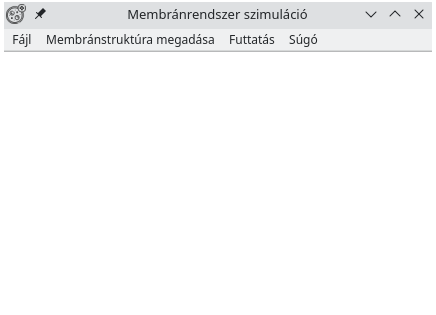
\includegraphics{main_window_empty.png}
	\caption{A főablak az alkalmazás megnyitásakor}
	\label{fig:main_window}
\end{figure}

A főablak az alkalmazás megnyitásakor még tartalmaz egyetlen grafikus elemet sem, viszont a menüsorban található menüpontok segítségével könnyedén változtatni lehet ezen. Ha a felhasználónak nincs korábbi tapasztala a program használatával, akkor érdemes a \textit{Súgó} menüpont kiválasztásával kezdenie, amelyről részletesen szó esik a \ref{help} fejezetben.

\subsection{Dialógusablakok}

A legfontosabb interakció a felhasználó és a szoftver között a dialógisablakokon keresztül történik.  

\subsubsection{Membránstruktúra megadása}\label{create_structure}

Egy membránrendszer megalkotásának kezdeti módja a struktúrájának megadásával kezdődik. Mivel egy membránrendszerben a membránok hierarchikusan helyezkednek el, ezért a teljes rétegződést nagyon jól lehet ábrázolni fa alakban, ahol mindenkinek a szülő csúcsa az őt legszűkebben tartalmazó régió. Ezzel egyenértékű az a felírás, amikor egyetlen karakterláncban fejezzük ki ugyanezt, azáltal, hogy egy régiót megfeleltetünk egy nyitó-csukó zárójelpárral. Ilyenkor a két zárójel között elhelyezett objektumok jelentik a régió tartalmát. Azonban nem csak objektumok, de más régiók is helyet kaphatnak, ezzel kifejezve azt, hogy a már említett régió közvetlen gyerekét szeretnénk megadni. 

\begin{figure}[H]
	\centering
	\subcaptionbox{Dialógusablak alapmodell létrehozásához}{
		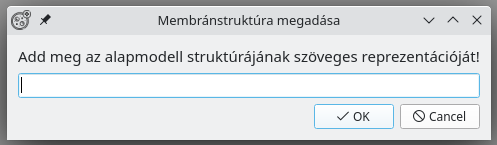
\includegraphics[width=0.45\linewidth]{structure_dialog_base_model.png}}
	\vspace{5pt}
	\subcaptionbox{Dialógusablak szimport-antiport rendszer létrehozásához}{
		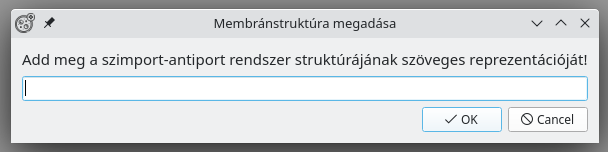
\includegraphics[width=0.45\linewidth]{structure_dialog_symport.png}}
	\caption{Dialógusablakok membránrendszer létrehozásához}
	\label{fig:create_system}
\end{figure}

A \ref{fig:create_system} ábra a különböző típusú membránrendszerek struktúrájának megadásához használt dialógusablakot mutatja. A megadott karakterláncban a régiók kezdetét és végét jelző zárójelpárok, illetve a bennük előforduló objektumok szerepelhetnek.
A helyes formátum feltétele, hogy a zárójelpárok karakterein és az szimport-antiport rendszereknél a kimeneti régió jelzésére használt speciális \textit{\#} karakteren kívül csak az angol ábécé kisbetűi szerepelhetnek a bemenetben, illetve annak meg kell felelnie a helyes zárójelezés szabályainak. Ezt azt jelenti, hogy nem lehetnek átfedések régiók között, azaz olyan karakterláncok, amikor egy külső régió hamarabb kerül lezárásra, mint bármelyik benne lévő régió. Ha ezen feltételeknek megfelel a felhasználó által megadott karakterlánc, akkor a főablak teljes területét lefedő vásznon megjelenik a létrehozott membránrendszer.

Ha a megadott karakterlánc nem a megfelelő formátumú, akkor a felhasználó figyelmeztetésére egy hibaüzenet jelenik meg a képernyőn. 

\subsubsection{Objektumok módosítása}

Miután a felhasználó megkonstruálta a membránrendszer szerkezetét, utána lehetősége nyílik arra, hogy az egyes régióinak tartalmát szerkessze. Mivel minden egyes régióhoz tartozhatnak objektumok és szabályok is egyaránt, ezért ezek módosítása közös dialógusablakban hajtható végre. A dialógusablak megjelenése a szerkeszteni kívánt régió által lefedett területre történő dupla kattintással kezdeményezhető. 

\begin{figure}[H]
	\centering
	\scalebox{0.8}[0.8]{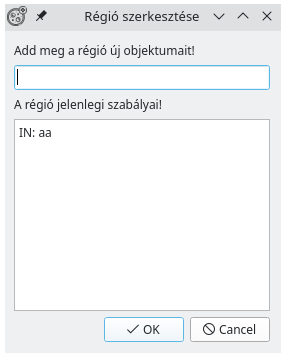
\includegraphics{rule_and_object_edit.png}}
	\caption{Dialógusablak egy régió tartalmának szerkesztéséhez}
	\label{fig:obj_edit}
\end{figure}

A régió objektumai közé tetszőleges számban írható a szóköz, mint elválasztó karakter, amely nem kerül figyelembevételre a régió új objektumainak feldolgozásakor. A megengedett karakterek ezen felül továbbra is az angol ábécé kisbetűi. Ha az adott régió a dialógusablak megnyitásakor már rendelkezik objektumokkal, akkor azok alapértelmezett szövegként fognak szerepelni a szövegdobozban. Tehát ha a régió szerkesztésekor az a felhasználó célja, hogy a kiválasztott régió tartalmát újabb objektumokkal egészítse ki, abban az esetben elegendő a hozzáadni kívánt karakterek begépelése.

\subsubsection{Szabályok módosítása}

A \ref{fig:create_system} segítségével alkotott membránrendszerek még nem fognak szabályokat tartalmazni, ám ezek nélkül nem beszélhetünk még szimulációról.  A szabályok fontos szerepet kapnak az információáramlás vezérlésében, hiszen a hatásukra tudnak objektumok átalakulni, be- és kivándorolni a régiók között. 

\begin{figure}[H]
	\centering
	\subcaptionbox{Régió szabályainak szerkesztése alapmodellben\label{fig:rule_edit_base}}{
		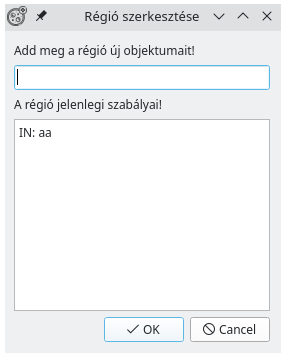
\includegraphics[width=0.45\linewidth]{rule_and_object_edit.png}}
	\vspace{5pt}
	\subcaptionbox{Régió szabályainak szerkesztése szimport-antiport rendszerben\label{fig:rule_edit_symport}}{
		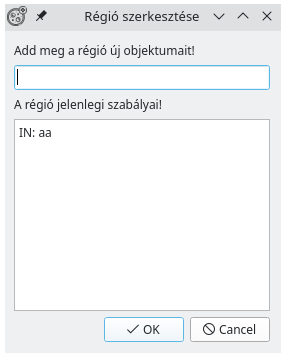
\includegraphics[width=0.45\linewidth]{rule_and_object_edit.png}}
	\caption{Membránrendszerek különböző formátumú szabályokkal}
	\label{fig:rule_edits}
\end{figure}

 A szabályok felépítése függ a membránrendszer típusától. Minden szabály megadása során először fel kell tüntetni, hogy mik azok az objektumok (olyankor ugyanolyan objektumból akár több is egyszerre), amelyek szükségesek a szabály alkalmazásához. 

Szimport-antiport rendszereknél ez a feltétel teljes mértékben elegendő ahhoz, hogy a szabály létrejöjjön, hiszen abban a modellben nincs lehetőség új objektumok létrehozására; a hangsúly inkább az objektumok régiók közötti mozgatására helyeződik. Ahogyan a \ref{fig:rule_edit_symport} alsó szövegdobozában is látható, szimport-antiport rendszerek esetében két típusú szabály hozható létre. Az első a szimport szabály, amelynek két formája van. Az \textit{IN:} kezdetű szabály alkalmazása esetén a kijelölt objektumok a membránt körülvevő tartományból a jelenleg szerkesztés alatt álló tartományba vándorolnak. Az \textit{OUT:} kezdetű szabálynál pedig a szerkesztés alatt álló régióból a membránt körülvevő tartományba kerülnek az objektumok.

\subsubsection{Szimulációk számának megadása}
\subsubsection{Mentés}
\subsubsection{Betöltés}
\subsubsection{Eredményablak}

\section{Használati útmutató}\label{help}